% 图契约：本题的源、边界和推导逐项对应；箭头符号按图注解释。
\documentclass[tikz,border=7pt]{standalone}
\usepackage{fontspec,xeCJK,amsmath,amssymb}
\IfFontExistsTF{Times New Roman}{\setmainfont{Times New Roman}}{\setmainfont{TeX Gyre Termes}}
\IfFontExistsTF{Heiti SC}{\setCJKmainfont[AutoFakeBold=1.5]{Heiti SC}}{\setCJKmainfont[AutoFakeBold=1.5]{FandolHei-Regular}}
\usetikzlibrary{arrows.meta,bending,calc,patterns,positioning}
\definecolor{ink}{HTML}{243745}
\definecolor{blue}{HTML}{275DAB}
\definecolor{green}{HTML}{177C63}
\definecolor{red}{HTML}{BD4935}
\definecolor{orange}{HTML}{AA6C16}
\definecolor{purple}{HTML}{715393}
\tikzset{every node/.style={font=\fontsize{9.3}{12.5}\selectfont,text=ink},
axis/.style={-{Stealth[length=4pt]},line width=.65pt,draw=ink!65},
vec/.style={-{Stealth[length=5pt]},line width=1pt,draw=blue},
short/.style={-{Stealth[length=3pt]},line width=.8pt},
guide/.style={dashed,draw=ink!40,line width=.5pt},
card/.style={rounded corners=2pt,draw=blue!65,fill=blue!4,align=center,text width=6.5cm,inner xsep=9pt,inner ysep=7pt},
title/.style={font=\fontsize{10.5}{14}\selectfont\bfseries,text width=15cm,align=center},
label/.style={font=\fontsize{8.4}{11}\selectfont,align=center},
note/.style={label,text width=6.2cm}}
\usepackage{unicode-math}\IfFontExistsTF{STIX Two Math}{\setmathfont{STIX Two Math}}{\setmathfont{Latin Modern Math}}
\begin{document}
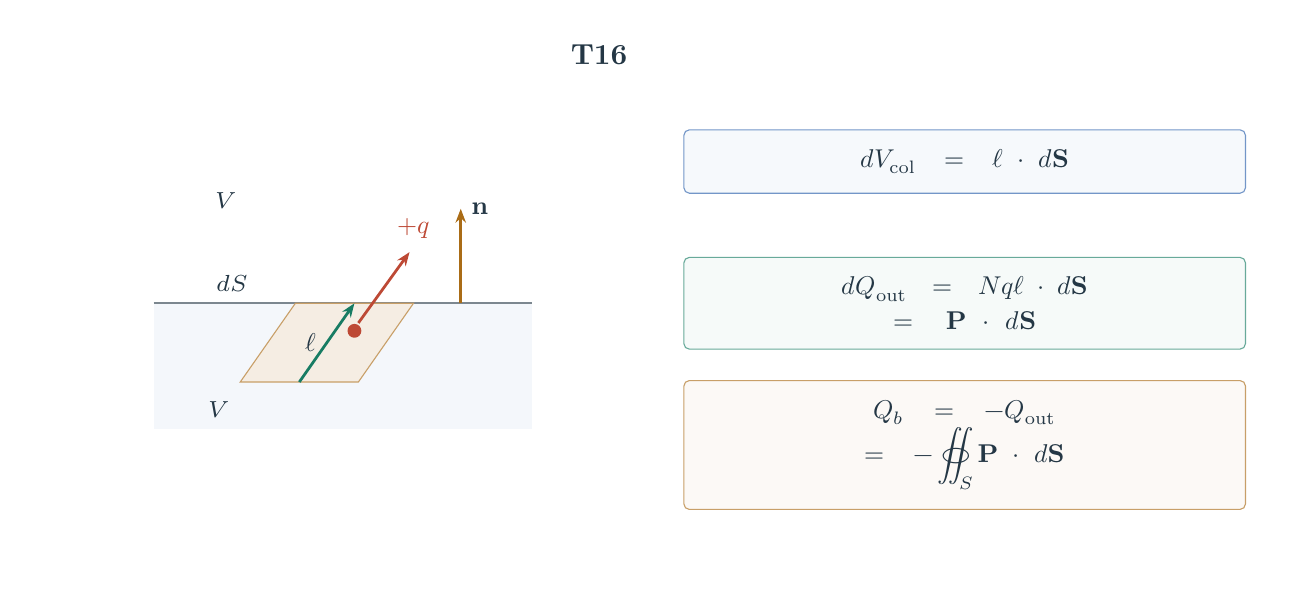
\begin{tikzpicture}[x=1cm,y=1cm]
\path[use as bounding box] (-8,-3.5) rectangle(8,3.5);
\node[title] at (0,3.15) {理论图 T16\quad 极化通量与闭合体积内留下的电荷};
\begin{scope}[shift={(-4,0)}]

\fill[blue!5] (-2.4,-1.6) rectangle(2.4,0);
\draw[ink!60,thick] (-2.4,0)--(2.4,0);
\filldraw[draw=orange!65,fill=orange!12] (-1.3,-1)--(.2,-1)--(.9,0)--(-.6,0)--cycle;
\draw[vec,green] (-.55,-1)--(.15,0) node[midway,left] {$\boldsymbol\ell$};
\draw[vec,orange] (1.5,0)--(1.5,1.2) node[right] {$\mathbf n$};
\node[label] at(-1.55,.25){面元 $dS$};
\node[label] at(-1.65,-1.35){体积 $V$ 内};\node[label] at(-1.55,1.3){体积 $V$ 外};
\fill[red](.15,-.35)circle(2.5pt);\draw[vec,red](.2,-.25)--(.85,.65);
\node[red] at(.9,.95){$+q$};
\node[note] at(0,-2.65){只有贴近边界且能穿出面元的正电荷，才贡献穿出通量。};
\end{scope}
\node[card,draw=blue!65,fill=blue!4] at (3.9,1.8) {$dV_{\rm col}=\boldsymbol\ell\cdot d\mathbf S$};
\node[card,draw=green!65,fill=green!4] at (3.9,0) {$dQ_{\rm out}=Nq\boldsymbol\ell\cdot d\mathbf S$\\$=\mathbf P\cdot d\mathbf S$};
\node[card,draw=orange!65,fill=orange!4] at (3.9,-1.8) {$Q_b=-Q_{\rm out}$\\$\displaystyle=-\oiint_S\mathbf P\cdot d\mathbf S$};
\end{tikzpicture}\end{document}